\documentclass{article}
\usepackage{graphicx} % Required for inserting images
\usepackage{placeins}


\title{Research Idea Matthijs Muis}
\author{Matthijs Muis}
\date{April 2023}


\usepackage{multicol}
\usepackage[utf8]{inputenc}     % for éô
\usepackage[english]{babel}     % for proper word breaking at line ends
\usepackage[a4paper, left=1in, right=1in, top=1in, bottom=1in]{geometry}
                                % for page size and margin settings
\usepackage{amsmath,amssymb}    % for better equations
\usepackage{amsthm}             % for better theorem styles
\usepackage{mathtools}          % for greek math symbol formatting
\usepackage{enumitem}           % for control of 'enumerate' numbering
\usepackage{listings}           % for control of 'itemize' spacing
\usepackage{todonotes}          % for clear TODO notes
\usepackage{hyperref}           % page numbers and '\ref's become clickable

%% SET TITLE PAGE VALUES HERE 
\def\thesistitle{Improving action sampling and removing the needs for complex constraints in Reinforcement Learning agents for HVAC control using Model-Predictive Controllers}
\def\thesisauthorfirst{Matthijs Muis}


%% FOR PDF METADATA
\title{\thesistitle}
\author{\thesisauthorfirst}
\date{May 19, 2023}


%% THEOREM STYLES
\newtheorem{theorem}{Theorem}[section]
\newtheorem{corollary}{Corollary}[theorem]
\newtheorem{lemma}[theorem]{Lemma}
\newtheorem{proposition}[theorem]{Proposition}

\theoremstyle{definition}
\newtheorem{definition}[theorem]{Definition}

\theoremstyle{remark}
\newtheorem*{remark}{Remark}


%% MATH OPERATORS
\DeclareMathOperator{\supersine}{supersin}
\DeclareMathOperator{\supercosine}{supercos}


%% SHORTCUT NOTATIONS
\newcommand{\mar}{\mathcal{M}}
\newcommand{\stat}{\mathcal{X}}
\newcommand{\act}{\mathcal{A}}
\newcommand{\prob}{\mathcal{P}}

\newcommand{\N}{\mathbb{N}}
\newcommand{\R}{\mathbb{R}}

%%%%%%%%%%%%%%%%%%%%%%%

\begin{document}
\maketitle
\tableofcontents

\newpage

\section{Outline of the problem}
\subsection{Topic}
In 2016, Deepmind reported that through application of its artificial intelligence technologies, it had been able to reduce the power consumption of Google's data centers by 40 \% \cite{evans_gao_2016}. Given the state-of-the-art efficiency of Google's data centers at the time, this meant a major breakthrough in the theory of control systems. The algorithm used reinforcement learning (RL) to learn the complex dynamics of the data center's cooling system. Another algorithm was developed in a more general datacenter setting \cite{gamble_gao_2018}. Later, Deepmind refocused on heating, ventilation and air-conditioning (HVAC) control systems and developed a deep reinforcement learning (DRL) controller named BCOOLER \cite{luo2022controlling}. 

Traditional HVAC control systems typically rely on simple feedback loop heuristics, called the \textit{sequence of operations} (SOO). These heuristics are sometimes based on predictions from an additional physical model for heat transport in the building, in which case we speak of model-predictive control (MPC) \cite{Schwenzer_Ay_Bergs_Abel_2021}. Heuristic models have simple feedback loop policies that misses many physical dynamics \cite{killian2016ten, Schwenzer_Ay_Bergs_Abel_2021}. MPC uses a hand-crafted physical model of the building, which often picks up no more complex dynamics than those envisioned by the designers \cite{luo2022controlling}. Despite succesful applications of MPC such as shown in \cite{privara2011modeling}, the downside is the difficulty of designing them. What is more, these models fail to take into account important non-physical influences such as building occupancy \cite{killian2016ten}. 

In contrast, an RL algorithm in principle requires no assumptions on the internal physical model of the data center: it learns optimal control actions directly from its interaction with the system. This was observed when Google's datacenter algorithm took ``advantage of winter conditions and produce colder than normal water, which reduces the energy required for cooling within the data centre'' \cite{gamble_gao_2018}. The potential of the RL framework has been noticed: Yu et al. report a surge of interest of the application of, in particular, Deep RL to autonomous HVAC control \cite{Yuetal}.

\subsection{Knowledge gap}
There are however still many barriers to take before the RL approach to HVAC controllers can become a mainstream framework. \cite{luo2022controlling} mentions as future work ``adding additional domain specific inductive biases to the model, such as the physical topology of the equipment in the facility, or the constraints and invariances of the sensor measurements given by first principle physics''. Current approaches to reinforcement learned HVAC control are model-free, which means that the agent has no internal model of the environment it interacts with: it has to map potential actions and states directly to its approximation of the action-value. Only then it can decide which action has the highest predicted action-value. Sampling sufficient actions becomes difficult due to the dimensionality of the problem.

This ``tabula rasa'' approach has the potential to increase the efficiency of the facility, if it works, but since it relies on opaque neural networks (in Deep RL, DRL) to approximate value-functions, its parameters have almost no interpretation. That is why it remains unclear whether they might generalize to other facilities. Moreover, their poor explainability makes it that they have no contribution to the current body of scientific knowledge when they fail to improve power efficiency.

Moreover, training of a model-free agent is difficult to do in a live environment, due to the invasiveness of training sessions for building occupants and equipment. Most of the research mentioned in \cite{Yuetal} in fact never sees the ``real world'', the RL agents being trained and evaluated all in a simulated environment. Deepmind's papers are quite unique in this aspect. \cite{evans_gao_2016, gamble_gao_2018, luo2022controlling} pre-train the agents on offline data collected from the existing SOO, and then complete the model by fine-tuning it in an online session by \textit{constrained reinforcement learning} (CRL) under safety constraints. An ironic point is that much time was spent on the design of constraints, while the motivation for using a model-free agent rather than a hand-crafted physical model is exactly to spend less time on the model design.

While constrained reinforcement learning is an active area of research \cite{agarwal2020optimistic}, as is offline reinforcement learning, \cite{levine2020offline}, little research has explored the potential of integrating a predictive model inside the RL agent (such as described in \cite{Seita_2019}) to , at least not in HVAC applications. MPC incorporates its constraint into a to be optimized cost function (see \ref{theory:HVAC}), so no complex constraints need to be formulated. It is based on a predictive model that can be pre-trained using supervised learning, meaning that training the agent using online RL is much less invasive, because it mostly involves fine-tuning control parameters. However, the model does not predict its future cost, meaning that there is little learning from the environment.

As we will see in the theoretical framework, the theories of RL and MPC show great similarity. It would be interesting to investigate more efficient sampling using a predictive model, and whether this improves the speed of convergence on a policy, and whether this improves the policy compared to a simple SOO in general. This is an excellent topic of further investigation, because even if the first experiments are not quite successful, it will still lay the foundation for the unification of the theory of MPC with RL. We can already rely on a rich body of theory involving model-based reinforcement learning, e.g. from the sources mentioned in \cite{Seita_2019}, so this is not at all an infeasible goal

These and other motivations, such as potential environmental benefits will be further explored under \ref{motivation}.

\subsection{Problem formulation}

We propose a novel approach to RL HVAC control that uses an agent that has an internal predictive model for the states, like in the theory of MPC, as well as an action-value approximator as in RL. The key difference is in the sampling of possible actions: these are sampled from a smaller space of actions that optimize the cost function (which is an explicit but non-probabilistic formulation of the action value coming from MPC theory). After designing a set of architectures for the predictive model, we train these using RL and benchmark against an existing SOO, both at a live facility and in a simulated environment. 

\paragraph{In brief} We design the hybrid MPC/RL controller $A$ using an intermediate predictive physical model $B$ in two stages. $B$ is a convolutional neural network that has in its local receptive fields inputs from sensors, actuators and demand-setters (i.e. thermostats that are set by building occupants) from space blocks that are adjacent, along with an input for day-of-week and time-of-day to predict occupancy. For the architecture of $B$ and $C$, we take inspiration from BCOOLER \cite{luo2022controlling}. The details can be found under \ref{Method:setup} and \ref{Method:modelA}, \ref{Method:modelling:B}.
\FloatBarrier
\begin{figure}
    \centering
    \includegraphics{Untitled Diagram.drawio.png}
    \caption{Diagram showing the outline of the hybrid MPC/RL model $A$}
    \label{fig:my_label}
\end{figure}
\begin{enumerate}
    \item \emph{Supervised stage:} Let $B$ learn to predict the future state $x_{t+1}$ from current state $x_t$ and action taken $a_t$, based on historical sensor data from the facility and a simulation model of the facility. This is a regression task which can be accomplished by analyzing static, offline data.
    \item \emph{Transfer reinforcement learning stage} Let $A$ be the model-predictive controller consisting of $B$, a (quadratic) loss function $J$ (as described under \ref{theory:HVAC}, and a model-free action-value predictor $C$ to evaluate sampled action-values. Its inputs connected to the sensors of the facility go to $B$ and feed back into $C$, the optimally picked action outputs to its HVAC equipment. Train $A$ in a simulated HVAC environment, and later in the live facility. The agent works as follows: first, sensor input enters the agent via $B$ and also via $C$. $B$ uses this to make predictions up to a horizon, given also the currently set actions from $J$. Given this new prediction horizon, $J$ is optimized in the fashion of MPC theory. This generates a set of optimal actions according to $J$, which is a more efficient sample of actions than just a random sample (and this is especially helpful in a high-dimensional actions space). Each action from the set is evaluated using an action-value predictor $C$, which utilizes the probabilistic approach from RL theory. The optimal action is selected and applied to the system. $C$ is much more complicated than $J$, but they both estimate the same action value. The difference is that $J$ is optimized analytically while $C$ is optimized by sampling solutions, which come from the neighbourhood of best solutions given by $J$.
\end{enumerate}

The aim is to create a framework that is generalizable to generic architectures for $B$ and thus to facilities, while also requiring as little online training and constraint formulation as possible by utilizing a predictive model that can be trained offline. The framework should improve the energy efficiency of a HVAC system that is noninvasive and thus affordable, also on smaller scales than those of Google's data centers.

\subsubsection{Research question}

The main research question can be summarized as: \\
\textit{How will the energy efficiency of the HVAC installation of a medium-sized building change compared existing SOO with the above proposed method, and how will the parameters of model $B$ change during the RL session? }

\subsubsection{Symmetry of outcomes}
Although the most interesting scenario would be to see the model perform better than the original SOO, the scenario of the  would not be useless. That is because we are developing a new framework, which can always be reused with a new predictive model substituted for $B$. Moreover, since $B$ is trained supervisedly, it is not difficult, invasive or expensive to retrain $B$. 

Also, the MPC agent $A$ is easier to interpret than a model-free agent, because we can clearly distinguish which part of the agent does the prediction and which part the decision making. So if $A$ fails to perform better, we can meaningfully analyze the trace of its parameters. Maybe $B$ did not converge, or overfit during training, being swung up and down by the changing of seasons which the orginal SOO was insensitive to. Or we may discover a new unthought-of cause. Either way, the trace of the parameters of $A$ (and $B$) will contribute to the current body of knowledge by providing future attention points to scientists and engineers who want to experiment with this approach.

\subsubsection{Subquestions}
These include:
\begin{enumerate}
    \item Which choice of model architecture for $B$ and the predictive heads of $B$ works best.
    \item How to mitigate the risk of users of the building through appropriate constraints while also maintaining good exploration during the RL stage, and mitigating the number of interupts due to constraint violations.
\end{enumerate} 
The above subquestions show that the product of this research is to improve a methodology

\subsection{Motivation} \label{motivation}
\paragraph{Door to small-scale optimization of HVAC control.}
Unlike existing research into RL control for HVAC, the new methodology does not intend to discard the predictive model that is central to MPC. The data-intensive part of this proces lies not in the RL stage but in the supervised stage: it utilizes RL only to tune the parameters. This makes the development of the model much less invasive, and requires considerably less thinking about the constraints and suitable constrained-RL methods. 

If succesful, the approach to training RL algorithms studied in this research could open the door to a generic, simplified method for partial on-line training of RL HVAC controllers in applications. The potential of these adaptive controllers has been shown in the aforementioned research, but seems to be limited to companies who can afford this approach by their scale, such as Google with its datacenters, having a large expenditure on cooling. This makes the main-stream application of these controllers still far away if the training process cannot be simplified dramatically.

\paragraph{Environmental impact}
HVAC systems make up a large portion of the energy consumption (EC) and greenhouse gas (GHG) emission of commercial buildings, and estimatedly 98\% of EC and GHG emission is from the lifetime of operational energy and not from the manufacturing and production energy \cite{co2emissionsfromhvacequipment,COLE1998335,SUZUKI199833,lifecycleenergyanalysis}. In 2016, energy use in commercial buildings made up for 6.6\% of global GHG emissions \cite{owidco2andgreenhousegasemissions}. Space cooling in general accounts for 10\% of the global electricity demand \cite{futureofcooling}. Improvements such as reported in \cite{evans_gao_2016} would mean a great benefit to the environment, but we repeat that the deployment of these algorithms needs to be simplified in order for them to become mainstream.



\paragraph{Model transparency and interpretation.}
As discussed above, the seperation of decision-making and prediction inside the agent makes it possible to assign meaning to the parameters the physical model learnt. $B$ might also correct for, and point out, sensor miscalibrations \cite{luo2022controlling} in the existing installation.

\section{Theoretical framework}

\subsection{HVAC control systems}\label{theory:HVAC}
We first introduce some useful terminology regarding space heating and cooling, which can be found in chap. 18 of \cite{ashraeHandbook}:

\paragraph{\textit{Load}} is the internal energy that needs to be removed from or added to the atmosphere in order to satisfy the current demand.

\paragraph{\textit{Wet-bulb temperature (WBT)}} Traditionally read by a thermometer covered in water-soaked cloth over which the air is passed. At 100\% air humidity, the WBT equals the temperature, otherwise it is lower than the actual air temperature. WBT is an accurate measure for how much cooling is necessary because it takes into account \textit{latent internal energy} contained in the water vapor in the air.

\paragraph{\textit{Capacity}} of an HVAC installation is the maximum load per unit time that the installation can remove from any space.

The energy-efficiency of an HVAC controller is measured its energy consumption per load removed. This efficiency depends highly on the cooling strategy, e.g. much energy can be saved by the correct use of a heat pump to store and reuse removed load.

\subsubsection{SOO types}
An HVAC installation is typically controlled by a rule-based control system called the \textit{sequence of operations} (SOO). This system can turn on pieces of equipment and can provide \textit{setpoints} to them. These setpoints are target values to be achieved on the individual equipment level \cite{luo2022controlling}. Achievement of the target is thus delegated entirely to equipment, which usually accomplishes this through a feedback-loop system. 

The controller can only see the achieved value and setpoint, and usually receives new measurements of these discrete time intervals. For large numbers of equipment, the total number of combinations of setpoints suffers from the curse of dimensionality \cite{luo2022controlling}, i.e. the action space gets very large. 

\subsubsection{Heuristic types}
Several types of heuristics exist that the SOO can be based on: these are listed from simplest to most advanced:

\FloatBarrier
\begin{figure}
    \centering
    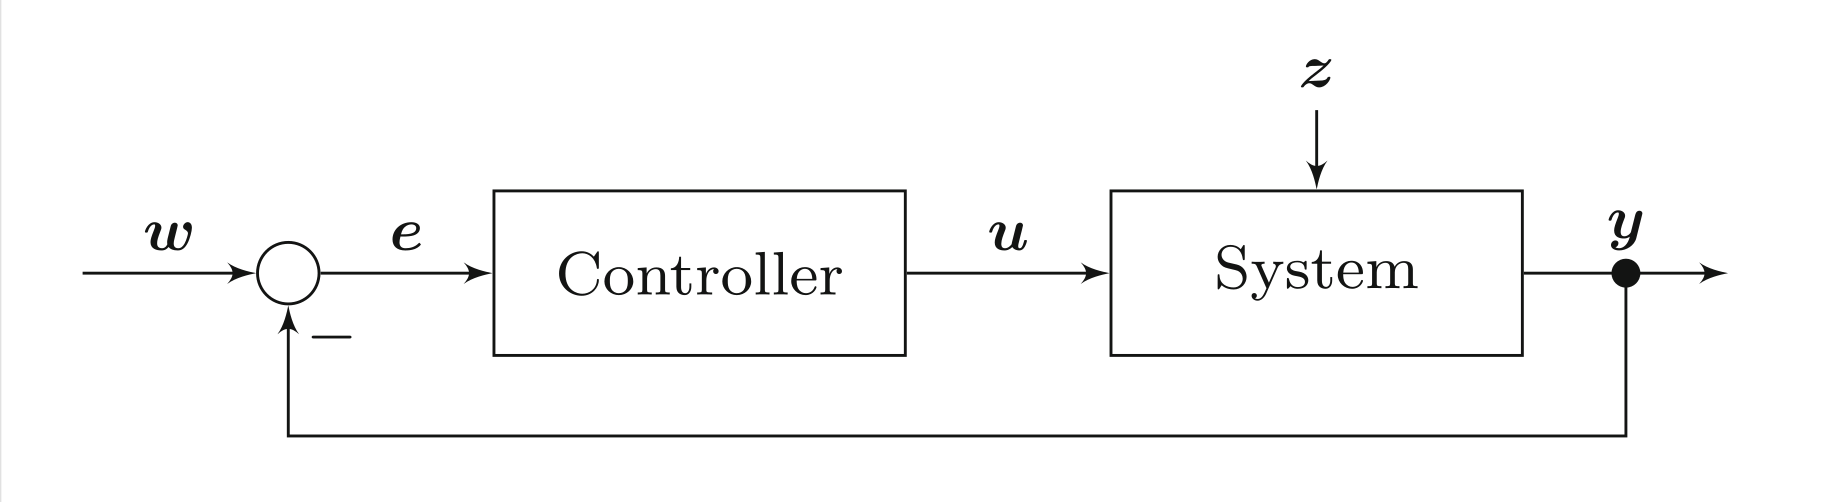
\includegraphics{feedbackloop.png}
    \caption{A simple feedback-loop controller, such as a PID controller. Source: \cite{Schwenzer_Ay_Bergs_Abel_2021}}
    \label{fig:my_label}
\end{figure}


\paragraph{Direct feedback-loop}: The difference between the demanded control variable value and the actual control variable value determines the setpoint of the equipment \cite{Schwenzer_Ay_Bergs_Abel_2021}.. An advanced example of this is the PID-controller (PID standing for Proportional, Differential, Integral).


\FloatBarrier
\begin{figure}
    \centering
    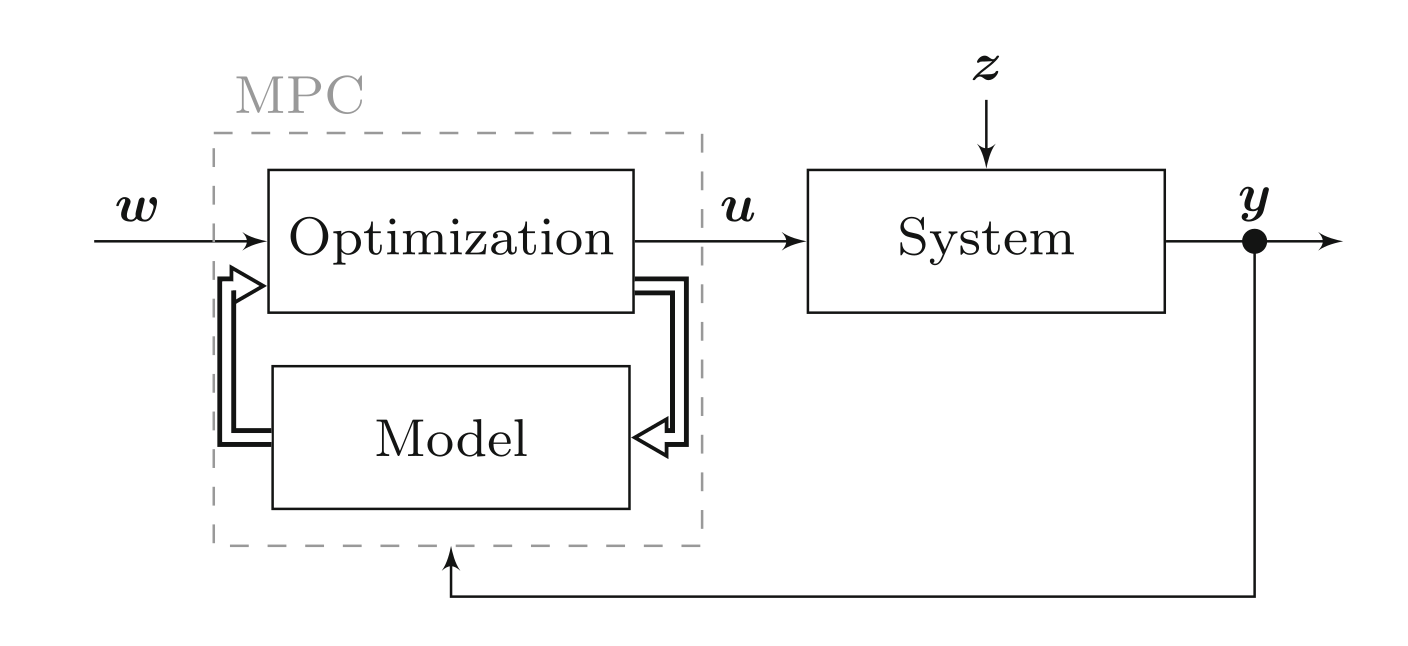
\includegraphics[width=1in]{mpc.png}
    \caption{An MPC controller. Source: \cite{Schwenzer_Ay_Bergs_Abel_2021}}
    \label{fig:my_label}
\end{figure}

\paragraph{MPC-based}
Our new RL agent will be built around an existing MPC controller. In MPC, the task of predicting the future state of the system based on action and current state is given to a separate predictive physical model \cite{privara2011modeling}, which has a role comparable to that of the critic in the actor-critic RL method \cite{suttonbarto2018, Szepesvari2010}. The SOO is split up in two separate parts: a predictive physical model maps the current state and control variables, say $x_t$ and $a_t$, to the predicted next state, $x_{t+1}$. Model $B$ is thus a function:
\begin{equation}
    x_{t+1} = B(x_t,a_t)
\end{equation}
The aim is then to minimize a cost function $J$ of the action $a$, parametrized bythe demand/reference $s_t$ and the predicted state $x_t$ and , summed over a ``finite horizon'' of future states, i.e.:
\begin{equation}
    \min_a \sum_{t=t_0}^{t_0+T}J(a, x_t, s_t)
\end{equation}
We use different letters for the variables than conventional literature (e.g. \cite{Schwenzer_Ay_Bergs_Abel_2021}) to emphasize the relationship with RL, which is discussed below
Constraints can be added if necessary, although these can also be included as penalty factors in $J$, see e.g. the function in \cite{privara2011modeling}. The parameters of the cost function and the constraints depend on the predicted future states, so the optimization and decision making (picking the optimal control variables $a_t$) come after the prediction made by the physical model. 


\FloatBarrier
\subsection{Reinforcement learning}

Reinforcement learning (RL) studies machine learning in the framework of a Markov decision process (MDP)
We will simply focus on the terminology and notation here. A detailed exposition of MDPs, RL and 
algorithms can be found in \cite{suttonbarto2018} and \cite{Szepesvari2010}

\begin{definition} A Markov decision process (MDP)  $\mar$ is a triple $\mar = (\stat, \act, \prob)$
Where $\stat$ is a countable set, also called the \emph{state space}, $\act$ is a countable set of actions and $\prob: \stat \times \act \rightarrow (\stat \times \R \rightarrow [0,1])$, $\prob: (x,a) \mapsto \prob_{(x,a)}$ a \emph{probability kernel} that assigns to every pair in $(x,a) \in \stat \times \act$ a probability measure $\prob_{(x,a)}:\stat \times \R \rightarrow [0,1]$. We denote the stochastic variable distributed according to $\prob_{(x,a)}$ as $(X,R)$ and it is further assumed that $R$ is bounded almost surely.
\end{definition}
This is the definition given in \cite{Szepesvari2010}.
Note that the definition imposes countability on the state and action space, which makes it
easier to define general algorithms for these models.

The interpretation of $\mar$ is as follows: for each state $x\in\stat$ an \emph{agent} can choose any
action from $\act$ and this gives a probability distribution over pairs of $(x,r)$ where $x\in\stat$ 
is the next state of the system and
$r\in \R$ is the immediate \emph{reward} the agent receives. 

Many problems that involve sequential 
decisions can be modeled by an appropriate state-reward space. By the definition, the model
assumes that the distribution for next state-reward pairs will only depend on the current state and
action taken. This property is referred to as the \emph{Markov} property of the model. Often when modelling
problems as MDPs one simly assumes this property or defines the state space such that each
state $x\in \stat$ also keeps the appropriate details of the history of the process up to the current state.

The goal one hopes to achieve is to find a strategy or policy $\pi : \stat \rightarrow \act$ such that if in
every state $x\in\stat$ the agent picks policy $\pi(x)$, the maximum achievable expected long-term reward is achieved. Generalizing further, the policy should sometimes be defined as a probability measure $\pi_x:\act \rightarrow [0,1]$ if the agent has to act unpredictably in order to play optimally. This is the case in a suitable
MDP model of the
game of rock, paper, scissors, for example. In HVAC controller systems, it is usually preferred that at least the controller itself behaves deterministically.

The goal of maximizing the expected reward can be formalized as follows:

\begin{definition} Given an MDP $\mar=(\stat,\act,\prob)$ and a (deterministic) policy $\pi$, the MRP $\mathcal{R}^pi$ is a tuple $(\stat, \prob^\pi)$ where $\prob^\pi:\stat\rightarrow \stat\times\R$ is the probability kernel given by $x\mapsto \prob_{(x,\pi(x))}$.
\end{definition}

\begin{definition} Fix a $\gamma \in ]0,1[$. The \emph{value} $V:\stat \rightarrow \R$ of an MRP $\mathcal{R}$ is given as:
\begin{equation}
V(x) = \mathbb{E}\left[ \sum_{t=0}^\infty \gamma^tR_{t+1} \ \vert \ X_0  = x\right]
\end{equation}
Where the sequences $(X_t)_{t\in\N}$, $(R_t)_{t\in\N}$ denote the stochastic sequences that are induced by $P$, where $X_t$ denotes the state at time $t\in\N$. These are determined entirely by the conditional distributions
\begin{align*}
    (X_t,R_t)|(X_j=x_j,R_j=r_j)_{j=0,..t-1}  &\sim (X_t,R_t)|(X_{t-1}=x_{t-1}) \\ (X_t,R_t)|(X_t=x_t) &\sim \prob_x
\end{align*}
\end{definition}

We can extend this definition to MDPs:

\begin{definition}
Fix a $\gamma \in ]0,1[$. The \emph{value} $V^\pi:\stat \rightarrow \R$ of the MDP $\mathcal{M}$ is given by
the value function $V$ of the MRP $\mathcal{R}^\pi$
\end{definition}

The final useful definitions involving policies and values:

\begin{definition}
Fix a $\gamma \in ]0,1[$. The \emph{action-value} $Q^\pi:\stat \times \act \rightarrow \R$ of the MDP $\mathcal{M}$ is given as:
\begin{equation}
Q^\pi(x,a) = \mathbb{E}\left[ V^\pi (X_1) + R_1 \ \vert \ (X_1,R_1) \sim \prob_{(x,a)}\right]
\end{equation}
Again, here we let $((X_t,A_t,R_{t+1})_{t\in \mathbb{N}}$ denote the stochastic process.
\end{definition}

Solving an MDP means: to find a policy $\pi$ that maximizes $V^\pi$ uniformly over $\stat$. The value of such a policy is $\pi^*$ is written as $V^*$ and called the \textit{optimal value function}. It satisfies, by definition:
\begin{equation}
  V^*(x) = \max_{\pi\in\Pi} V^\pi(x)  
\end{equation}
Where $\Pi$ denotes the set of all stochastic stationary policies \cite{Szepesvari2010}. We see that this equation is only sensible when the policy $\pi^*_x$ that maximizes the right hand side is the same for all states $x$, because this is what, by definition, \textit{uniform} maximization over $\stat$ requires. 

Analogously to $V^*$, we can define the \textit{optimal action-value function} $Q^*$ of $(x,a)\in \stat \times \act$ as the optimal value plus expected immediate reward given state $x$ and action $a$.

\subsubsection{Additional notation}

\paragraph{Transition probability} The probability measure $\prob$ gives rise to a state transition probability $\prob : \stat \times \act \times \stat \rightarrow [0,1]$ which assigns to every triple $(x,a,y)$ the probability that the system transitions to state $y$ given action $a$ and current state $x$.

\paragraph{Expected reward (1)} For every pair $(x,a)\in \stat \times \act$ we can define ${r(x,a) := \mathbb{E}[R_{t+1} \ | \ X_t = x, A_t = a]}$. Note that this is well defined due to time-homogeneity of the process.

\paragraph{Expected reward (2)} For every pair $x\in \stat$ we can define ${r(x) := \mathbb{E}[R_{t+1} \ | \ X_t = x]}$. Again, this is well defined due to time-homogeneity of the process.

\subsection{Reinforcement learning algorithms}
\subsubsection{Optimality as a fixed point}

Uniform maximization is possible in the more well-behaved class of MDPs when we allow for the aforementioned stochastic policy type \cite{Szepesvari2010}. Let $Y^X$ denote the set of all functions $X\rightarrow Y$. Also, let $r(x,a)$ When dealing with not all too exotic MDPs  we are concerned with deterministic policies, we see that in general $Q^\pi$ and $\pi$ need to satisfy the \textit{Bellman Equation} \cite{suttonbarto2018, Szepesvari2010}:
\begin{align}
    T^\pi Q^\pi &= Q^\pi \\
    T^*Q^* &= Q^*
\end{align}

Where we define $T^\pi, T^*$ as $\R^{\stat\times \act} \rightarrow \R^{\stat\times \act}$: 
\begin{align}
    (T^\pi Q)(x,a) &:= r(x,a) + \gamma \sum_{y\in \stat} \prob(x,a,y)Q(y,\pi(y)), & (x,a)\in \stat \times \act \\
    (T^* Q)(x,a) &:= r(x,a) + \gamma \sum_{y\in \stat} \prob(x,a,y)\sup_{a'\in \act}Q(y,\pi(y)), & (x,a)\in \stat \times \act
\end{align}

Further, we note that it is enough to know $Q^*$ to deduce $\pi^*$, as:
\begin{align}
    \pi^*(x) &= \text{arg}\max_{a\in \mathcal{A}} Q^* (x,a), &\forall x \in \mathcal{X}
\end{align}

\subsubsection{Policy iteration}
The problem here is that the terms on both sides depend on $\pi^*$, which needs to be found. The method of policy iteration approaches the problem of solving this equation for $\pi^*$ as follows:

\begin{enumerate}
    \item \textit{Action-value estimation:} Simulate of the MRP given by the MDP followed under $\pi_k$. This is followed by an appropriate (statistical) estimation $\hat Q^\pi_{k+1}$ of the function $Q^\pi$ for a current policy $\pi_k$.
    
    \item \textit{Policy update:} Find the new $\hat\pi_{k+1}$ that is optimal with respect to the newly estimated $\hat Q^\pi_k$.
\end{enumerate}

The intuitive idea is that every iteration $k$ $\hat Q^\pi_{k}$ will be more accurate, meaning that the policy $\hat\pi_k$ can be estimated closer to $\pi^*$, which in turn implies that $\hat Q^\pi_{k+1}$ will resemble $Q^*$ more closely. The circular argument is noticeable. Yet, various theorems from the field show that under regularity conditions this process does indeed converge on some fixed points for $Q$ and $\pi$, which in the case of the right choice of parametrization (i.e. model architecture) for $\hat Q$ and $\hat\pi$ would indeed approximate the optimal action-value and optimal policy.

 

When the action and/or state space is high-dimensional, it is often infeasible to keep an estimation of $Q(x,a)$ and $\pi(x)$ for every pair $(x,a) \in \stat\times\act$, the so-called \textit{tabular approach} \cite{suttonbarto2018, Szepesvari2010}. The alternative approach considered in this research, \textit{value-function approximation} is to parametrize the policy $\pi$ through a parameter $\mu$ and parametrize the value function $Q^\pi$ through a parameter $\theta$, and then to iteratively:
\begin{enumerate}
    \item \textit{Action-value estimation:} Simulate of the MRP given by the MDP followed under $\pi_k$. This is followed by an appropriate (statistical) estimation of the parameter $\theta$ to improve the estimate $\hat Q^\pi_{k+1}$ of the function $Q^\pi$ for a current policy $\pi_k$.
    
    \item \textit{Policy update:} Find a new value of parameter $\mu$ that optimizes $\hat\pi_{k+1}$ with respect to the newly estimated $\hat Q^\pi_k$.
\end{enumerate}

There are many variants on both action-value estimation and policy-update methods, of which a detailed exposition can be found in \cite{suttonbarto2018, Szepesvari2010}. The algorithm proposed in our research will be discussed under \ref{Method:RLAlg}.


\section{Method}
The method can be separated into a design phase and an experimentation phase. Subsections \ref{Method:FeatureSel},\ref{Method:MDP},\ref{Method:modelling:B},\ref{Method:modelA},\ref{Method:RLAlg} detail on the design phase while subsections \ref{Method:DatC}\ref{Method:DatAn} detail on the experimental setup. Subsection \ref{Method:setup} discusses both aspects.
\subsection{Setup}\label{Method:setup}
We will train the agent in the Mercator II building of Radboud University Nijmegen. This is a multi-tenant office building, housing companies with a close connection to the Faculty of Science of this university \cite{MercatorSciencePark_2023}. This choice has several reasons:

\begin{enumerate}
    \item The researcher is a student of Radboud University and expects the building tenant to be open for student innovation in the realm of energy-saving. 
    \item The design of the building had energy-efficiency in mind from the inception of the plan, see e.g. the project description of the architect, \cite{PauldeRuiter_2023} Because of this, we expect smaller noise in the HVAC demand than in conventional buildings. This has several potential benefits.
    
    First, it means that random confounders (i.e. open windows, doors) if they arise, do not lead to such high variance in performance variables as in buildings not designed with these influences in mind. 
    This is beneficial because mitigating the influence of confounders, means our measurements of the performance difference between the extension and the original become more accurate. 
    
    Second, a conciously energy-efficient design might mean a higher density of sensors and actuators, which will allow us to collect more relevant data and give the model a finer control of the environment.

    Third, we hope that the energy-efficient design also comes with an extensive SOO for the HVAC control of the building.
    
    \item The building houses offices only, in contrast to e.g. the Huygens building on the same campus, which has added demand in cooling and heating from its many laboratories.
\end{enumerate}

The building has a bruto floor area of 7.000 m$^2$, and has the uniform shape of an elongated cube. Designed by Paul de Ruiter architects, its (HVAC) equipment is due to Boonstoppel Engineering and Deerns \cite{PauldeRuiter_2023}. In order to make a model of the building together with its different space blocks, sensors, actuators and thermostats, we will need to consult these three parties. We also need to discuss with them the heuristics underlying the original SOO, and ask about the availability of historical data collected by this SOO.

Further, if not present we need to install sensors on the outside of the walls of the building. This is because we want to collect data from the environment of the building in order to better model the heat flow. This is also done because the environment temperature of the building can be a confounder when comparing performances of $A$ against $B$ (see \ref{Method:DatAn:confounders}

\paragraph{SOO requirements} we do require the SOO to have an internal MPC model, as this will provide the basis foro model $B$, which is a predictive physical model . We also require the model to be differentiable with respect to its parameters, because it would complicate the policy iteration of $A$ dramatically if this is not the case.

If the provided SOO does not satisfy this requirement, we must arrange an SOO that is differentiable, and we must also arrange an additional MPC model. Of these two models, we then have to reshape the input/output topology of this SOO such that it fits the sensor/actuator topology of the experimental setup. The new parameters of this imported SOO MPC controller do not have to be trained before the conversion to model $B$ and $A$. We will benchmark the final model against power consumption data of the original SOO of the facility.

\subsection{Observed features}\label{Method:FeatureSel}

The system will then be modeled as follows:
First, the internal space of the building is partitioned in segments that correspond with spaces that have restricted air flow between them. The goal of this is that sensors, actuators and demand-setters (i.e. thermostats that are set by building occupants) from space blocks that are adjacent should be modeled as \textit{local receptive fields} in the CNNs that form the architecture of model $B$. The reason for this approach are detailed under \ref{Method:modelling:B}. 

We also require every demand-setter to be paired with a sensor, since we need to calculate the difference between the demanded temperature and the achieved temperature. This is typically already the case as every piece of equipment typically relies on a feedback-control loop to achieve and maintain its setpoint. Finally, we require a time-of-day and day-of-week input for the models, which can be provided by a timing function in the computer system where the models are trained.

We expect the available sensors to measure the variable in which demands are expressed, namely air temperature, but also other variables such as humidity and possibly air pressure, to infer the WBT as a more accurate measure of load. These measurements are typically collected at discrete, regular time intervals (see \ref{theory:HVAC} which provides a natural discretization of the timeline for the MDP. We should collect what quantities are measured and in what units. We expect the original control system to already provide us with a central interface to collect this sensory data.


\subsection{Simulation environment}
In order to let $B$ learn offline and train $A$, we will make a model of the Mercator II building, if not provided by the engineers of Boonstoppel or Deerns. This can be done in one of the many software packages available to this end, such as the open-source software package HVACSIM+ developed by the NIST \cite{Galler_2021}. Since the tool is quite complex and the designer has probably already done work on it, we definitely need to consult the engineering team for Mercator II on their modelling work.

\subsection{MDP formulation} \label{Method:MDP}
\subsubsection{State space}
The states $x_t\in \mathcal{X}$ are defined as $N+4$-tuples of the form ${x_t = ((L^n\textbf{T}_t)_{n=0,1,..N}, (L^n\textbf{D}_t)_{n=0,1,..N}, \textbf{S}_t, \tau_t)}$. This representation contains:
\begin{enumerate}
    \item $\textbf{S}_t \in \mathbb{R}^d$, a vector of $d$ demanded setpoints from thermostats in the building. These are all demands expressed as a temperature.
    \item All temperature sensor data $\textbf{T}_t \in \mathbb{R}^d$ received from $d$ sensors that are paired to the $d$ thermostats in the building. These pairs are selected based upon distance between the setter and sensor. Of both $\textbf(S)$ and $\textbf{T}$, the last $n$ measurement instances preceding $t$, along with a vector of setpoints $\textit{S}_t$ demanded from the thermostats. Here, we use the convenient notation $L$ for the \textit{lag operator} $LT_t := T_{t-1}$. $N$ is a to be determined hyperparameter \footnote{With this, we assume that the process is Markovian with respect to this state space, which might approximately hold if we include enough lagged sensor measurements of previous time intervals. The choice of the hyperparameter $N$ leads to a trade-off between data and dimensionality, which has to be delved into deeper during the design. One can separate the observations from the state-space, which gives rise to a so-called Partially Observed MDP (POMDP). However, this is rarely done in practice since it complicates the model quite a lot. This proposal uses ``observation'' and ``state'' interchangeably}
    \item Sensory data $\textbf{D}_t \in \mathbb{R}^p$, which is the vector into which all other sensor measurements are collected. These include temperature data from sensors that could not be paired to a thermostat, but also sensors for humidity. Like $\mathbf{T}$, the state is determined by both current measurements as lagged measurements $L^n\mathbf{D}_t$.
    \item The time-of-day and day-of-week timings collected in $\tau_t\in \{0,1,..24\}\times \{1,2,..7\}$
\end{enumerate}
The temperature will first be normalized as to WBT so that the predictive model $B$ receives physically sensible input data. This will later make it easier to interpret its parameters as representing physical constants of proportionality.

\subsubsection{Action space}\label{MDP:actions}
As discussed under \ref{theory:HVAC}, the control system can only influence the HVAC system by turning on and of pieces of equipment (actuators) in certain places and providing a setpoint for them. The way of achieving the setpoint is delegated to the local equipments, which usually uses a feedback loop for this \footnote{This usually implies that actuators for heating are paired with a sensor for heat in the vicinity, and the same goes for AC actuators and humidity and temperature sensors.}. The action space $\act$ thus consists of the cartesian product of consinuous ranges of setpoints, all ranges are paired with a binary variable that takes values in $\{$on, off$\}$. The exact ranges of setpoints along with minor alterations to the aforementioned structure depend on what we find when investigating the equipment.


\subsubsection{Rewards and constraints} \label{constraints}
The reward function is not directly trivial in this setting. The problem is that the agent has three objectives:
\begin{enumerate}
    \item Minimize the difference between the demanded WBT and the actual WBT,
    \item Minimize the total power consumption of the equipment per load,
    \item Control the equipment in a sustainable and careful way.
\end{enumerate}
An agent that prioritizes the first criterium will probably skyrocket Mercator's energy bill, while an agent that prioritizes the second will leave poor office workers in freezingly cold rooms on a wintry day. We follow the implementation of criteria that is presented in most literature: 
\begin{enumerate}
    \item \textit{The reward} is the negative of the total power consumption per estimated load of the HVAC equipment, $\frac{-P_t}{l(x_t)}$ (which must be maximized). Load calculation $l(x_t)$ is done by the simulation software based on first-principle physical formulas.
    \item  The deviation between thermostat setpoint and actual temperature $\mathbf{T}_{t+1}-\mathbf{S}_{t+1}$ of the next state should always be bounded, leading to a constraint on the future state distribution \cite{gamble_gao_2018, evans_gao_2016, luo2022controlling}. 
    \item Additional direct constraints on the actions $a_t$ should prevent unresponsible usage of the equipment, e.g. continuously turning on/off the AC. This second constraint type requires keeping track of past actions. But these past actions do not have to be part of the state representation, because the constraints are not part of the MDP. 
\end{enumerate}
    These constraints do not have to be implemented as constraints on the optimization criterion, but can also be added as penalty terms to the optimization criterium. This would \textit{change} the definition of the \textit{reward}. Since we can simulate and thus try many models, we can empirically test which $J$ yields fastest convergence and optimal efficiency. We do not have to dream these up ourselves, but can look at the conventional formulae for $J$ that are used in HVAC literature, and see whether the imported MPC already provides settings for this.


\subsection{General modelling considerations}
We want the architecture of $B$ to take into account the topology of the building: this is done through a convolutional neural networks (CNN). A convolutional neural network has, in contrast to a regular neural network, every neuron in the first hidden layer connected to only a small subset of adjacent neurons in the input layer. Such groups of neurons are called \textit{local receptive fields}, and their aim is to represent the topology or geometry of the input being analyzed: in our case, it does not make much sense to connect two sensor inputs from completely different parts of the building to the same hidden neuron, since the measurements from these sensors have no interesting relationship. However, it would be useful to investigate local relationships between adjacent rooms. 



\end{document}